\documentclass[a4paper, 11pt, normalem]{report}

\usepackage{../../../LaTeX-Templates/Notes}

\titlecontents{chapter}% <section-type>
    [0pt]% <left>
    {}% <above-code>
    {Lecture \thecontentslabel\quad}% <numbered-entry-format>
    {}% <numberless-entry-format>
    {\dotfill\contentspage}% <filler-page-format>
\titleformat{\chapter}{\fontsize{13}{15}\bfseries\normalfont}{\textbf{Lecture \thechapter}}{1em}{}
\titleformat{\subsection}{\fontsize{11}{15}\scshape}{\thesubsection}{1em}{}
\setcounter{tocdepth}{4}
% \setcounter{secnumdepth}{1}

\renewcommand{\arraystretch}{1.2}

\title{Mathematical Methods \\ In Physics \vspace{-20pt}}
\author{Dr Cristina Zambon}
\date{\vspace{-15pt}Michaelmas Term 2017}
\rhead{\hyperlink{page.1}{Go to TOC}}

\begin{document}

\maketitle
\tableofcontents

\chapter{}
\section{Geometrical Applications of Vectors in $\mathbb{R}^3$}
\begin{wrapfigure}{r}{0.4\textwidth}
    \begin{center}
        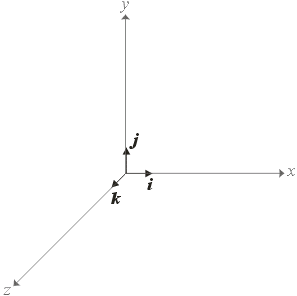
\includegraphics[scale=0.5]{Cart.png}
    \end{center}
\end{wrapfigure}
\begin{gather*}
    \vec{a} =
    \begin{pmatrix}
        a_1 \\
        a_2 \\
        a_3
    \end{pmatrix}
    \iff
    \vec{a} = a_{1}\hat{i} + a_{2}\hat{j} + a_{3}\hat{k} \\
    \vec{b} =
    \begin{pmatrix}
        b_1 \\
        b_2 \\
        b_3
    \end{pmatrix}
    \iff
    \vec{b} = b_{1}\hat{i} + b_{2}\hat{j} + b_{3}\hat{k}
\end{gather*}
We consider a cartesian system:

$\{\hat{i}, \hat{j}, \hat{k}\} = $ 'standard basis'

This set is an orthonormal set of vectors:

The vectors $\hat{i}, \hat{j}, \& \hat{k}$ are orthogonal and have a modulus of 1

\begin{equation*}
    \hat{i} \perp \hat{j};~~ \hat{i} \perp \hat{k};~~ \hat{j} \perp \hat{k}
\end{equation*}
\begin{equation*}
    |\hat{i}| = |\hat{j}| = |\hat{k}| =  1
\end{equation*}

\section{Scalar (or dot) Product}
\begin{wrapfigure}{r}{0.35\textwidth}
    \begin{center}
        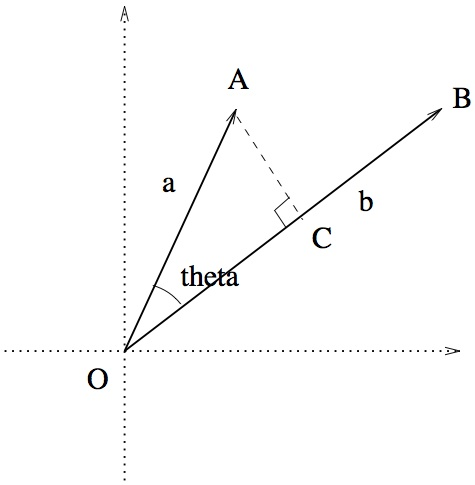
\includegraphics[scale=0.5]{Scalar.jpg}
    \end{center}
\end{wrapfigure}
\begin{gather*}
    \vec{a} \cdot \vec{b} = |\vec{a}||\vec{b}|\cos\theta \\
    \vec{a} \cdot \vec{b} = a_{1}b_{1} + a_{2}b_{2} + a_{3}b_{3}
\end{gather*}
$\vec{a}$ can be split into components $\perp$ and $\parallel$ to $\vec{b}$:
\begin{equation*}
    \vec{a} = \vec{a}_{\parallel} + \vec{a}_{\perp}
\end{equation*}
\begin{itemize}
    \item $\vec{a}_{\parallel} \equiv \vec{OC}$ is the orthogonal projection of $\vec{a}$ on to the direction of $\vec{b}$
    \item Its modulus is $|\vec{a}|\cos\theta = \frac{\vec{a} \cdot \vec{b}}{|\vec{a}|}$
\end{itemize}
\begin{equation*}
    \vec{a}_{\parallel} = \Bigg(\frac{\vec{a} \cdot \vec{b}}{|\vec{b}|}\Bigg) \frac{\vec{b}}{|\vec{b}|} \implies \vec{a}_{\perp} = \vec{a} - \vec{a}_{\parallel}
\end{equation*}
The dot product is symmetrical so:
\begin{gather*}
    \vec{a} \cdot \vec{b} = \vec{b} \cdot \vec{a} \\
    |\vec{a}| = \sqrt{\vec{a} \cdot \vec{a}}
\end{gather*}

\newpage
\section{Vector (or cross) Product}
\begin{wrapfigure}{r}{0.4\textwidth}
    \begin{center}
        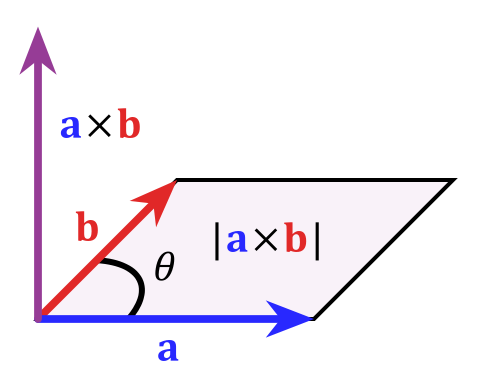
\includegraphics[scale=0.3]{Cross.png}
    \end{center}
    \vspace{-200pt}
\end{wrapfigure}
\begin{gather*}
    \vec{a} \times \vec{b} =
    \begin{pmatrix}
        a_1 \\
        a_2 \\
        a_3
    \end{pmatrix}
    \times
    \begin{pmatrix}
        b_1 \\
        b_2 \\
        b_3
    \end{pmatrix}
    =
    \begin{pmatrix}
        a_{2}b_{3} - a_{3}b_{2} \\
        a_{3}b_{1} - a_{1}b_{3} \\
        a_{1}b_{2} - a_{2}b_{1}
    \end{pmatrix} \\
    |\vec{a} \times \vec{b}| = |\vec{a}||\vec{b}|\sin\theta
\end{gather*}
Notice that $|\vec{a} \times \vec{b}|$ is the area of the parallelogram with sides $\vec{a}$ and $\vec{b}$

The cross product is anti-symmetric:
\begin{equation*}
    \vec{a} \times \vec{b} = -\vec{b} \times \vec{a}
\end{equation*}

\section{Scalar Triple Product}
\begin{equation*}
    [\vec{a}, \vec{b}, \vec{c}] = \vec{a} \cdot (\vec{b} \times \vec{c}) =
    \begin{vmatrix}
        a_1 & a_2 & a_3 \\
        b_1 & b_2 & b_3 \\
        c_1 & c_2 & c_3
    \end{vmatrix}
\end{equation*}
The absolute value of the scalar triple product for three arbitrary vectors $\vec{a}, \vec{b},$ and $\vec{c}$ corresponds to the volume of the parallelepiped with sides $\vec{a}, \vec{b},$ and $\vec{c}$
\begin{gather*}
    |[\vec{a}, \vec{b}, \vec{c}]| = |\vec{a}||\vec{b} \times \vec{c}|\cos\phi = |\vec{a}||\vec{b}||\vec{c}|\sin\theta\cos\phi
\end{gather*}
It is unchanged under an even permutation of the vectors:
\begin{equation*}
    [\vec{a}, \vec{b}, \vec{c}] = [\vec{b}, \vec{c}, \vec{a}] = [\vec{c}, \vec{a}, \vec{b}]
\end{equation*}
It changes sign under an odd permutation:
\begin{equation*}
    [\vec{a}, \vec{b}, \vec{c}] = -[\vec{b}, \vec{a}, \vec{c}] = -[\vec{a}, \vec{c}, \vec{b}] = -[\vec{c}, \vec{b}, \vec{a}]
\end{equation*}
It vanishes if any two vectors are the same

\section{Einstein Summation Convention for Subscripts}
\emph{Any index that appears twice in a given term of an expression is understood to be summed over all the values that an index can take}

The summed-over subscripts are called dummy subscripts and the others, free subscripts
\begin{gather*}
    \sum_{i = 1}^{n} a_{i}b_{i} \equiv a_{i}b_{i} \\
    a_{ij}b_{jk} = \sum_{j = 1}^{3} a_{ij}b_{jk} = a_{i1}b_{1k} + a_{i2}b_{2k} + a_{i3}b_{3k} \\
    a_{ij}b_{jk}c_{k} = \sum_{j = 1}^{3} \sum_{k = 1}^{3} a_{ij}b_{jk}c_{k} ~~~ \text{(Gives 9 terms)}
\end{gather*}

\section{Kronacker Delta in $\mathbb{R}^{3}$}
\begin{gather*}
    \delta_{ij} =
    \begin{cases}
        1 & \text{ if } i = j \\
        0 & \text{ otherwise}
    \end{cases}
    ;~~~ i,\,j = 1,\,2,\,3 \\
    b_{i}\delta_{ij} = b_{1}\delta_{1j} + b_{2}\delta_{2j} + b_{3}\delta_{3j}
    \begin{cases}
        j = 1 & \to ~ b_{1} \\
        j = 2 & \to ~ b_{2} \\
        j = 3 & \to ~ b_{3}
    \end{cases}
    \Bigg\} \implies b_{j} \\
    b_{i}\delta_{ij} = b_{j} \\
    \delta_{ii} = \delta_{11} + \delta_{22} + \delta_{33} = 3 \\
    \vec{a} \cdot \vec{b} = a_{i}b_{i} = \delta_{ij}a_{i}b_{j}
\end{gather*}

\section{Levi-Civita Symbol in $\mathbb{R}^3$}
\begin{gather*}
    \epsilon_{ijk} =
    \begin{cases}
        +1 & \text{if i,j,k is an even permutation of 1,2,3}       \\
           & \epsilon_{123} = \epsilon_{231} = \epsilon_{312} = 1  \\
        -1 & \text{if i,j,k is an odd permutation of 1,2,3}        \\
           & \epsilon_{213} = \epsilon_{132} = \epsilon_{321} = -1 \\
        0  & \text{otherwise}
    \end{cases}
\end{gather*}
\subsection{Features}
\begin{enumerate}
    \item $\epsilon_{ijk} = \epsilon_{jki}$ (even permutation) \\
          It does not change sign
    \item $\epsilon_{ijk} = -\epsilon_{jik}$ (odd permutation) \\
          It changes sign under the interchange of any pair of indices
    \item $\epsilon_{ijj} = \epsilon_{iii} = 0$
\end{enumerate}

\subsection{Exercises}
\begin{enumerate}
    \item $(\vec{a} \times \vec{b})_i = \epsilon_{ijk}a_{j}b_{k}$ \\
          $(\vec{a} \times \vec{b})_1 = \epsilon_{1jk}a_{j}b_{k} = \epsilon_{123}a_{2}b_{3} + \epsilon_{132}a_{3}b_{2} = a_{2}b_{3} - a_{3}b_{2}$
    \item $[\vec{a},\vec{b},\vec{c}] = \epsilon_{ijk}a_{i}b_{j}c_{k} =  a_{1}b_{2}c_{3} + a_{2}b_{3}c_{1} + a_{3}b_{1}c_{2} - a_{1}b_{3}c_{2} - a_{2}b_{1}c_{3} - a_{3}b_{2}c_{1}$
\end{enumerate}

\chapter{}
\section{Lines in $\mathbb{R}^3$}
\begin{wrapfigure}{r}{0.4\textwidth}
    \begin{center}
        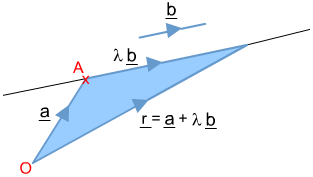
\includegraphics[scale=0.5]{EqLine.png}
    \end{center}
\end{wrapfigure}
Consider a point A and a direction $\hat{b}$:
\begin{gather*}
    (\vec{r} - \vec{a}) = \hat{b}\lambda \\
    \vec{r} = \vec{a} + \hat{b}\lambda
\end{gather*}
Note that $\vec{r} =\vec{r}(\lambda)$ (parametric form)

Note also that by taking the vector product with $\hat{b}$, we obtain another equation for the line:
\begin{equation*}
    (\vec{r} - \vec{a}) \times \hat{b} = 0
\end{equation*}

\section{Equation of a plane in $\mathbb{R}^3$}
\begin{wrapfigure}{r}{0.4\textwidth}
    \vspace{-20pt}
    \begin{center}
        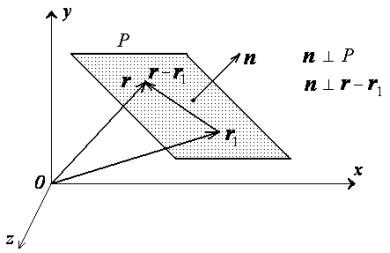
\includegraphics[scale=0.6]{Plane.jpg}
    \end{center}
    \vspace{-80pt}
\end{wrapfigure}
A plane through a point A with position vector, $\vec{a}$, and perpendicular to uni vector, $\hat{n}$, is:

\begin{gather*}
    (\vec{r} - \vec{a}) \cdot \hat{n} = 0 \\
    \vec{r} \cdot \hat{n} = \vec{a} \cdot \hat{n} = d
\end{gather*}
This is the Cartesian form for the equation of a plane

Consider a plane with points A, B, and C with corresponding position vectors:
\begin{equation*}
    t_{1}(\vec{b} - \vec{a}) + t_{2}(\vec{c} - \vec{a} = \vec{r} - \vec{a})
\end{equation*}
This is the parametric equation for a plane

\section{Linear Vector Spaces}
Found in Chapter 8 of Riley, Hobson, and Bence

A vector space, V, is a set whose elements are called "vectors" and such that there are two operations defined on them:
\begin{itemize}
    \item you can add vectors to each other
    \item you can multiply vectors by a scalar
\end{itemize}
Those operations must obey certain simple rules; these rules are called \emph{axioms} \\
The Axioms for a Vector Space are:
\begin{enumerate}
    \item The vector space is closed under addition and scalar multiplication
        \begin{itemize}
            \item If $\vec{v}$ and $\vec{u} \in$ V, then $\vec{v} + \vec{u} \in$ V
            \item If $\vec{v} \in$ V, then $\alpha\vec{v} \in$ V
        \end{itemize}
    \item Associativity
        \begin{itemize}
            \item $(\vec{u} + \vec{v}) + \vec{w} = \vec{u} + (\vec{v} + \vec{w})$
            \item $(\alpha\beta)\vec{v} = \alpha(\beta\vec{v})$
        \end{itemize}
    \item There exists a \emph{zero element} or \emph{neutral element}, $\vec{0}$
        \begin{itemize}
            \item $\vec{0} + \vec{v} = \vec{v}$
        \end{itemize}
    \item There exists an \emph{inverse element}, $-\vec{v}$
        \begin{itemize}
            \item $\vec{v} + (-\vec{v}) = \vec{0}$
        \end{itemize}
    \item Commutativity
        \begin{itemize}
            \item $\vec{u} + \vec{v} = \vec{v} + \vec{u}$
        \end{itemize}
    \item Distributivity
        \begin{itemize}
            \item $\alpha(\vec{v} + \vec{u}) = \alpha\vec{v} + \alpha\vec{u}$
            \item $(\alpha + \beta)\vec{v} = \alpha\vec{v} + \beta\vec{v}$
        \end{itemize}
    \item Scalar multiplication by 1 leaves $\vec{v}$ unchanged
        \begin{itemize}
            \item $1\vec{v} = \vec{v}$
        \end{itemize}
\end{enumerate}
Note that by scalar, we usually mean $\in \mathbb{R}$ \\
In this case, we refer to V as a \emph{real vector space}

It is also possible for scalars $\in \mathbb{C}$ \\
in this case, we have \emph{complex vector spaces}

\subsection{Examples}
\begin{enumerate}
    \item $\mathbb{R}$
    \item Generalisation to $\mathbb{R}^n$ for Euclidean vector spaces
    \item Further generalised to $\mathbb{C}^n$
    \item The set of all real functions, $f(x)$, with no restrictions on x and with the usual (calculus) addition and scalar multiplication
        \begin{itemize}
            \item $(f_1 + f_2 )(x) = f_{1}(x) + f_{2}(x)$
            \item $(\alpha f)(x) = \alpha f(x)$
        \end{itemize}
    \item The matrices of size $(n \times m)$ with real elements and the usual (calculus) addition and scalar multiplication of matrices
    \item The set of vectors in the 3D space for which $2X - 3Y + 11Z + 2 = 0$ \textbf{is not a vector space}
        \begin{itemize}
            \item $\vec{0} \notin$ V
            \item $2\cdot0 - 3\cdot0 + 11\cdot0 + 2 \neq 0$
        \end{itemize}
    \item $2X - 3Y + 11Z = 0$ is a vector space
    \item Consider a second order, linear, homogeneous differential equation of the form:
        \begin{itemize}
            \item $p(x)\frac{d^{2}f}{dx^2} + q(x)\frac{df}{dx} + r(x)f = 0$
            \item p, q, and r are fixed functions
        \end{itemize}
        The space of the solutions of such an equatino forms a vector space under the usual addition and scalar multiplication
\end{enumerate}






















\end{document}
